\chapter{Конструкторская часть}

\section{Разработка архитектуры системы}

Модуль трассировки лучей инкапсулирует вызовы C++ ядра, передавая конфигурацию сцены в виде структур данных и возвращая RGB-массивы освещенности. Вычислительный модуль (C++) выполняет трассировку лучей от источников света, расчет преломления в колпачках, определение пересечений с объектами сцены и формирование карт освещенности. Модуль визуализации преобразует предрассчитанные карты освещенности в изображения для отображения.

\subsection{IDEF0 диаграмма первого уровня (A0)}

\begin{figure}[H]
\centering
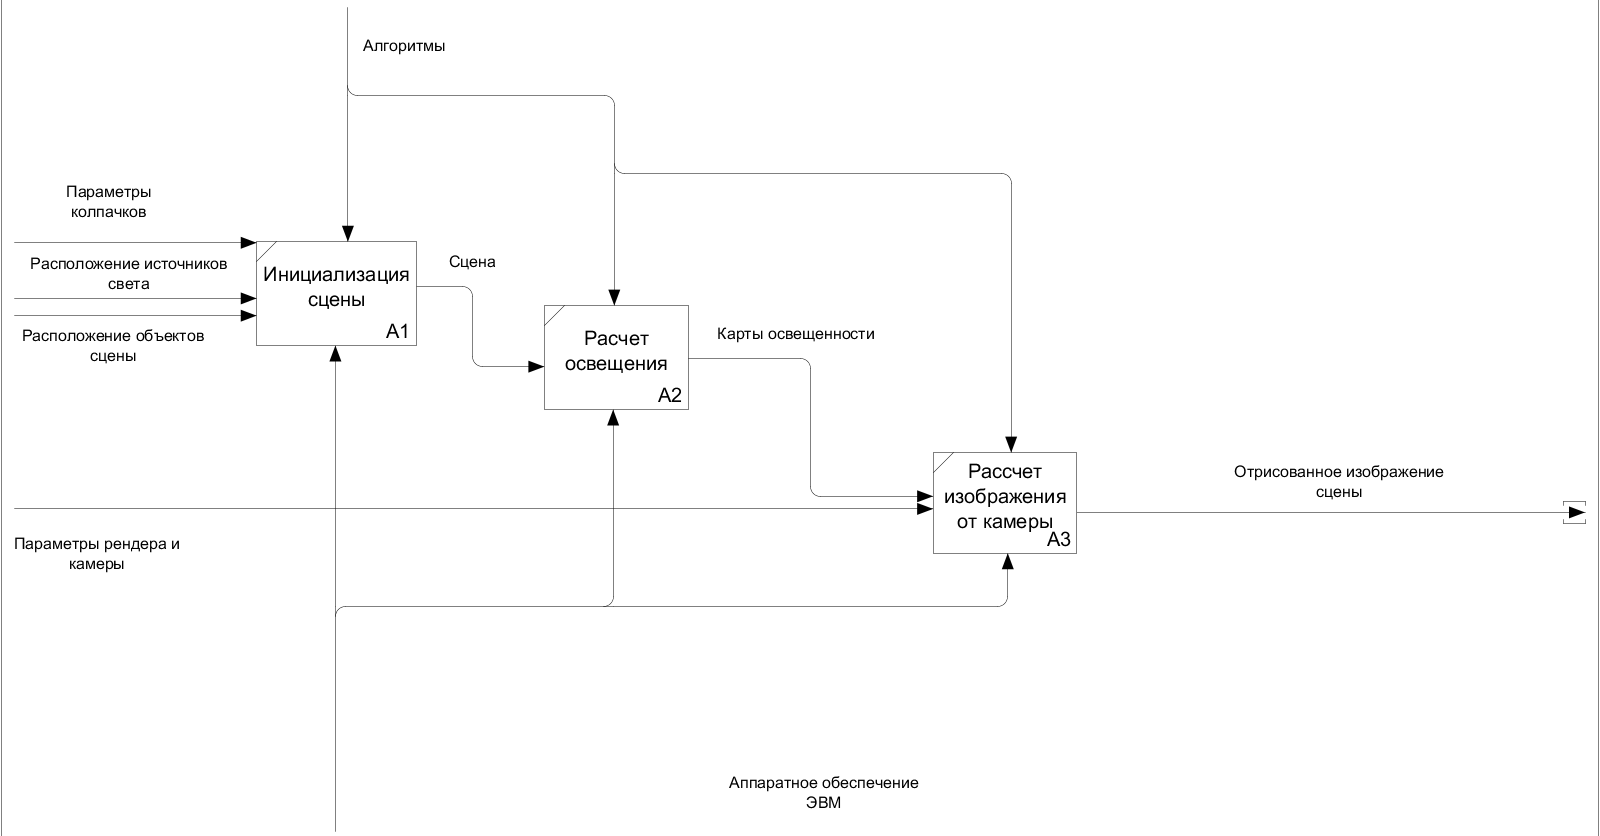
\includegraphics[width=1\textwidth]{images/02_A0.png} 
\caption{Диаграмма декомпозиции первого уровня (IDEF0 A0)}
\label{fig:idef0_a0}
\end{figure}

\section{Математическое описание}

\subsection{Модель освещения (Закон Ламберта)}

Для расчета интенсивности освещения используется модель диффузного отражения Ламберта \cite{3,7}:

\begin{equation}
I = I_0 \cdot \rho \cdot \max(0, \vec{n} \cdot (-\vec{d}))
\end{equation}

где:
\begin{itemize}
    \item $I$ --- результирующая интенсивность;
    \item $I_0$ --- интенсивность луча;
    \item $\rho$ --- коэффициент диффузного отражения (0--1);
    \item $\vec{n}$ --- нормаль к поверхности;
    \item $\vec{d}$ --- направление луча.
\end{itemize}

При накоплении освещенности от множества лучей:

\begin{equation}
I_{\text{total}} = \sum_{i=1}^{N} I_i
\end{equation}

где:
\begin{itemize}
    \item $I_{\text{total}}$ --- суммарная интенсивность освещения;
    \item $N$ --- количество лучей;
    \item $I_i$ --- интенсивность от $i$-го луча.
\end{itemize}

\subsection{Модель преломления (Закон Снеллиуса)}

Защитный колпачок источника света представляет собой сферический слой, состоящий из двух концентрических сфер с общим центром, но разными радиусами (внешняя и внутренняя сферы). Источник света расположен внутри малой сферы. При трассировке луча от источника происходит двойное преломление: сначала луч пересекает внешнюю сферу (вход в материал колпачка), затем внутреннюю сферу (выход из материала). Нормаль к поверхности в каждой точке пересечения вычисляется как нормаль к соответствующей сфере в этой точке.

При прохождении луча через границу раздела двух сред направление изменяется согласно закону Снеллиуса \cite{3}:

\begin{equation}
n_1 \sin(\theta_1) = n_2 \sin(\theta_2)
\end{equation}

где:
\begin{itemize}
    \item $n_1$ --- показатель преломления первой среды;
    \item $n_2$ --- показатель преломления второй среды;
    \item $\theta_1$ --- угол падения;
    \item $\theta_2$ --- угол преломления.
\end{itemize}

Вектор преломленного луча:

\begin{equation}
\vec{d}_{\text{refr}} = \eta \vec{d} + (\eta \cos(\theta_1) - \cos(\theta_2)) \vec{n}
\end{equation}

где:
\begin{itemize}
    \item $\vec{d}_{\text{refr}}$ --- направление преломленного луча;
    \item $\eta = n_1 / n_2$ --- отношение показателей преломления;
    \item $\vec{d}$ --- направление падающего луча;
    \item $\vec{n}$ --- нормаль к поверхности;
    \item $\cos(\theta_1) = -\vec{d} \cdot \vec{n}$ --- косинус угла падения;
    \item $\cos(\theta_2) = \sqrt{1 - \eta^2 (1 - \cos^2(\theta_1))}$ --- косинус угла преломления.
\end{itemize}

При $\eta^2 (1 - \cos^2(\theta_1)) > 1$ происходит полное внутреннее отражение.

\subsection{Аппроксимация Френеля (формула Шлика)}

Для моделирования отражения и преломления используется аппроксимация Шлика \cite{7}:

\begin{equation}
R_0 = \left(\frac{n_1 - n_2}{n_1 + n_2}\right)^2, \quad R(\theta) = R_0 + (1 - R_0)(1 - \cos(\theta))^5
\end{equation}

где:
\begin{itemize}
    \item $R_0$ --- коэффициент отражения при нормальном падении;
    \item $R(\theta)$ --- коэффициент отражения при угле падения $\theta$;
    \item $n_1$, $n_2$ --- показатели преломления двух сред;
    \item $\cos(\theta) = |\vec{d} \cdot \vec{n}|$ --- косинус угла падения.
\end{itemize}

Интенсивность преломленного луча:

\begin{equation}
I_{\text{refracted}} = I_{\text{in}} \cdot (1 - R)
\end{equation}

где:
\begin{itemize}
    \item $I_{\text{refracted}}$ --- интенсивность преломленного луча;
    \item $I_{\text{in}}$ --- интенсивность падающего луча;
    \item $R$ --- коэффициент отражения.
\end{itemize}

\subsection{Модель поглощения и фильтрации света}

Интенсивность луча уменьшается пропорционально прозрачности материала:

\begin{equation}
I_{\text{out}} = I_{\text{in}} \cdot (1 - \alpha), \quad \vec{C}_{\text{out}} = \vec{C}_{\text{in}} \odot \vec{C}_{\text{material}}
\end{equation}

где:
\begin{itemize}
    \item $I_{\text{out}}$ --- интенсивность выходящего луча;
    \item $I_{\text{in}}$ --- интенсивность входящего луча;
    \item $\alpha = 1 - \text{transparency}$ --- коэффициент поглощения;
    \item $\vec{C}_{\text{out}}$ --- цвет выходящего луча;
    \item $\vec{C}_{\text{in}}$ --- цвет входящего луча;
    \item $\vec{C}_{\text{material}}$ --- цвет материала;
    \item $\odot$ --- покомпонентное умножение RGB векторов.
\end{itemize}

\subsection{Модель рассеивания (матовость)}

Для имитации матовых колпачков используется упрощенная модель рассеивания, основанная на добавлении случайного возмущения к вектору преломленного луча:

\begin{equation}
\vec{d}_{\text{scattered}} = \text{normalize}(\vec{d}_{\text{refr}} + \vec{\xi}), \quad \xi_i \sim \mathcal{N}(0, \sigma^2)
\end{equation}

где:
\begin{itemize}
    \item $\vec{d}_{\text{scattered}}$ --- направление рассеянного луча;
    \item $\vec{d}_{\text{refr}}$ --- направление преломленного луча;
    \item $\vec{\xi}$ --- случайное возмущение;
    \item $\xi_i \sim \mathcal{N}(0, \sigma^2)$ --- компоненты возмущения, распределенные по нормальному закону;
    \item $\sigma$ --- параметр шероховатости материала.
\end{itemize}

Данная модель является упрощением более точных физических моделей рассеивания, таких как распределение GGX (Trowbridge-Reitz) или модель Блинн-Фонг, которые учитывают микрорельеф поверхности и обеспечивают более реалистичное распределение отраженного света. Упрощенная модель выбрана для обеспечения приемлемой производительности при расчете большого количества лучей, при этом она качественно воспроизводит эффект матовости для декоративных колпачков.

\subsection{Модель пересечения луча со сферой}

Для определения пересечения луча $\vec{P}(t) = \vec{O} + t \vec{d}$ со сферой $|\vec{P} - \vec{C}|^2 = R^2$ решается квадратное уравнение:

\begin{equation}
at^2 + bt + c = 0
\end{equation}

где:
\begin{itemize}
    \item $\vec{P}(t) = \vec{O} + t \vec{d}$ --- параметрическое уравнение луча;
    \item $\vec{O}$ --- начало луча;
    \item $\vec{d}$ --- направление луча;
    \item $t$ --- параметр луча;
    \item $\vec{C}$ --- центр сферы;
    \item $R$ --- радиус сферы;
    \item $a = 1$;
    \item $b = 2 \vec{d} \cdot (\vec{O} - \vec{C})$;
    \item $c = |\vec{O} - \vec{C}|^2 - R^2$;
    \item $D = b^2 - 4ac$ --- дискриминант.
\end{itemize}

При $D \geq 0$ точка пересечения: $t = \frac{-b - \sqrt{D}}{2a}$.

\subsection{Модель пересечения луча с плоскостью (стена)}

Для плоскости $\vec{n} \cdot \vec{P} = d$ параметр пересечения:

\begin{equation}
t = \frac{d - \vec{n} \cdot \vec{O}}{\vec{n} \cdot \vec{d}}
\end{equation}

где:
\begin{itemize}
    \item $t$ --- параметр точки пересечения;
    \item $\vec{n} \cdot \vec{P} = d$ --- уравнение плоскости;
    \item $\vec{n}$ --- нормаль к плоскости;
    \item $d$ --- расстояние от начала координат до плоскости;
    \item $\vec{O}$ --- начало луча;
    \item $\vec{d}$ --- направление луча.
\end{itemize}

Если $\vec{n} \cdot \vec{d} = 0$, луч параллелен плоскости. При $t > 0$ вычисляется точка пересечения.

\subsection{Модель распределения направлений лучей}

Стратифицированная сетка:

Для генерации $N$ направлений лучей создается сетка размером $G \times G$, где $G = \lfloor \sqrt{N} \rfloor$. Направления вычисляются по формулам:

\begin{equation}
\phi_i = \frac{i}{G-1} \cdot \pi, \quad \theta_j = \frac{j}{G-1} \cdot 2\pi
\end{equation}

где:
\begin{itemize}
    \item $\phi_i$ --- полярный угол для $i$-й строки сетки;
    \item $\theta_j$ --- азимутальный угол для $j$-го столбца сетки;
    \item $G = \lfloor \sqrt{N} \rfloor$ --- размер сетки;
    \item $N$ --- общее количество направлений;
    \item $i, j = 0, 1, \ldots, G-1$.
\end{itemize}

\begin{equation}
\vec{d}_{i,j} = (\sin(\phi_i) \cos(\theta_j), \sin(\phi_i) \sin(\theta_j), \cos(\phi_i))
\end{equation}

где:
\begin{itemize}
    \item $\vec{d}_{i,j}$ --- единичный вектор направления;
    \item $i, j = 0, 1, \ldots, G-1$ --- индексы сетки.
\end{itemize}

Сферическая решетка Фибоначчи:

Для $k$-й точки из $N$ точек направление вычисляется по формулам:

\begin{equation}
t_k = \frac{k + 0.5}{N}, \quad y_k = 1 - 2t_k, \quad r_k = \sqrt{1 - y_k^2}, \quad \theta_k = \varphi \cdot k
\end{equation}

где:
\begin{itemize}
    \item $t_k$ --- нормализованный параметр для $k$-й точки;
    \item $y_k$ --- координата $y$ на сфере;
    \item $r_k$ --- радиус проекции на плоскость $xz$;
    \item $\theta_k$ --- азимутальный угол;
    \item $k = 0, 1, \ldots, N-1$ --- индекс точки;
    \item $N$ --- общее количество точек;
    \item $\varphi = \pi(3 - \sqrt{5})$ --- золотой угол.
\end{itemize}

\begin{equation}
\vec{d}_k = (r_k \cos(\theta_k), y_k, r_k \sin(\theta_k))
\end{equation}

где:
\begin{itemize}
    \item $\vec{d}_k$ --- единичный вектор направления для $k$-й точки.
\end{itemize}


\subsection{Схемы основных алгоритмов}

\subsubsection{Алгоритм предварительного расчета освещения}

Выполняет трассировку лучей от всех источников света и формирует карты освещенности.

Входные данные: Конфигурация источников света, объектов сцены, параметры расчета.

Выходные данные: Карты освещенности для стены и сфер.

\begin{figure}[H]
\centering
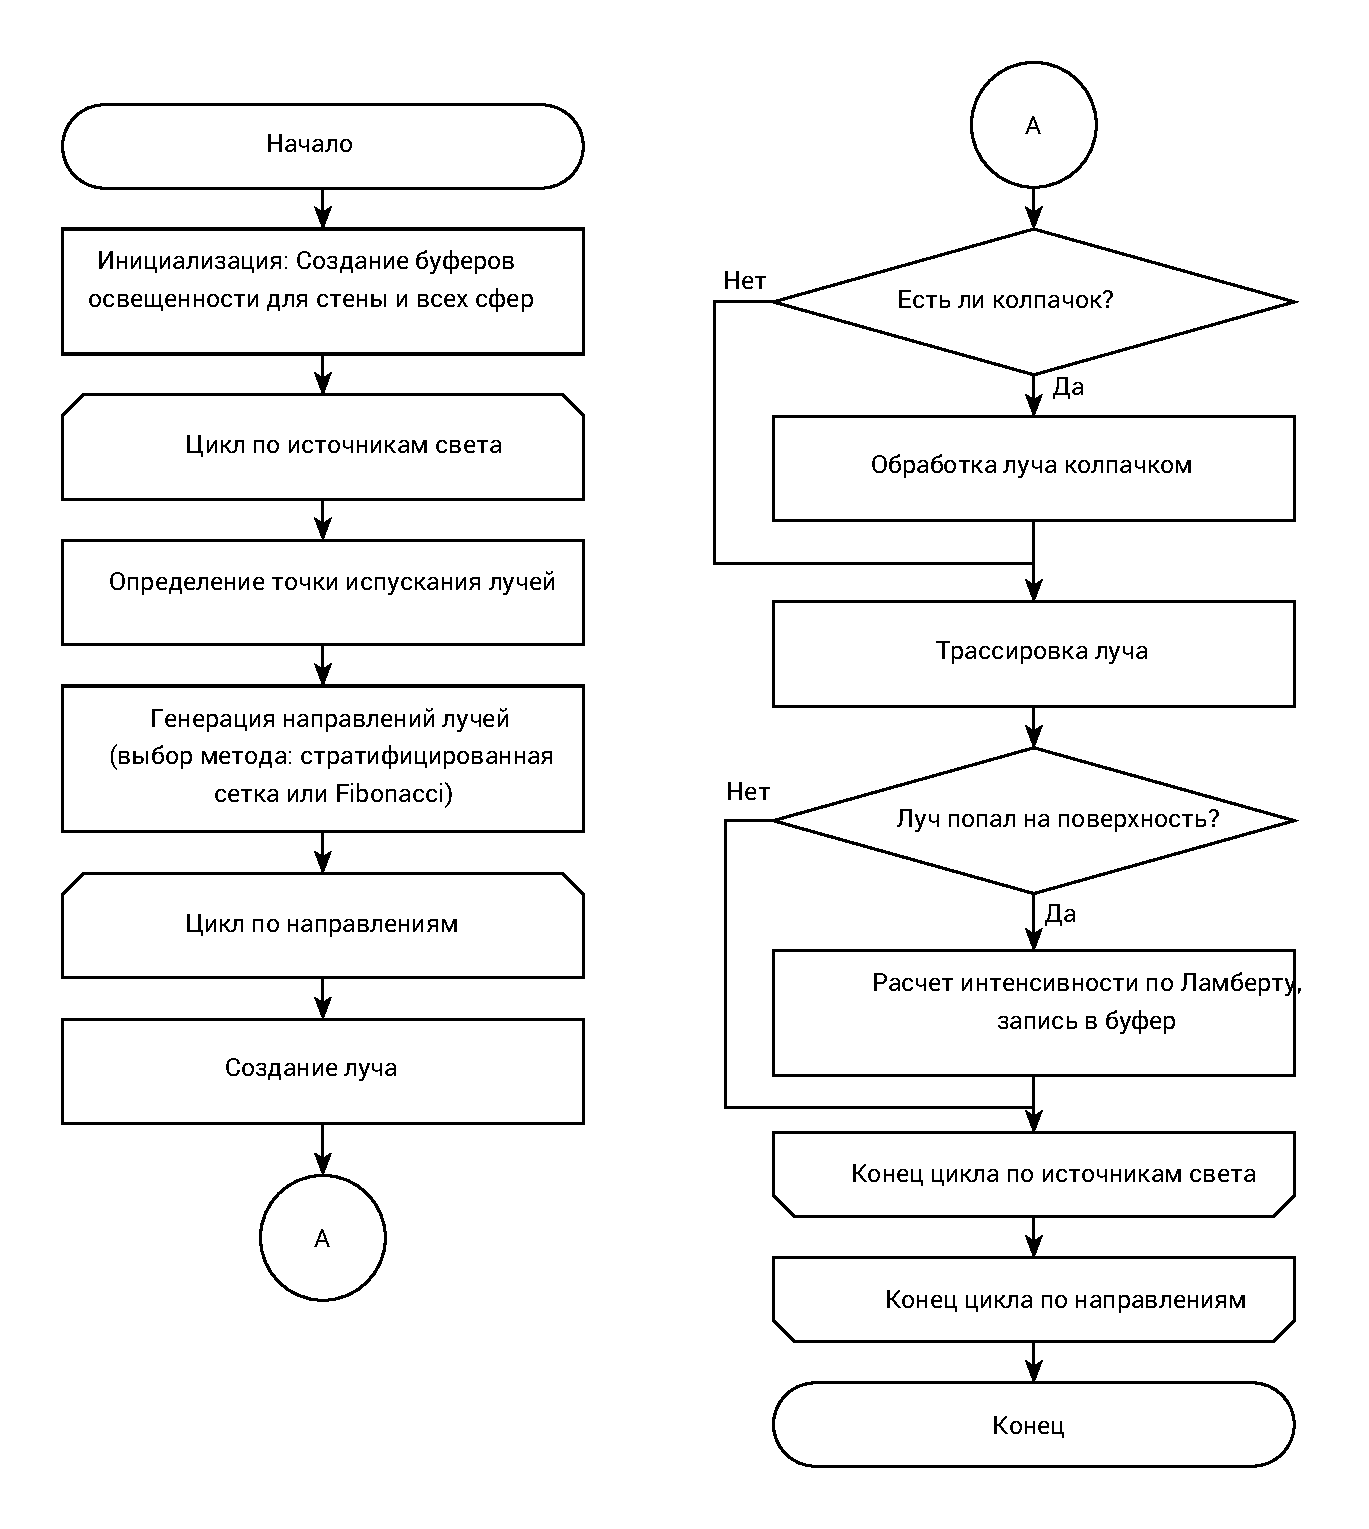
\includegraphics[width=0.9\textwidth]{images/algo_precalc.pdf}
\caption{Схема алгоритма предварительного расчета освещения}
\label{fig:algo_precalc}
\end{figure}

\subsubsection{Алгоритм трассировки луча}

Определяет ближайшее пересечение луча с объектами сцены и записывает вклад освещения в карту освещенности.

Входные данные: Луч (начало, направление, интенсивность, цвет), конфигурация объектов сцены.

Выходные данные: Обновленный буфер освещенности.

\begin{figure}[H]
\centering
% Здесь будет вставлена блок-схема алгоритма трассировки луча
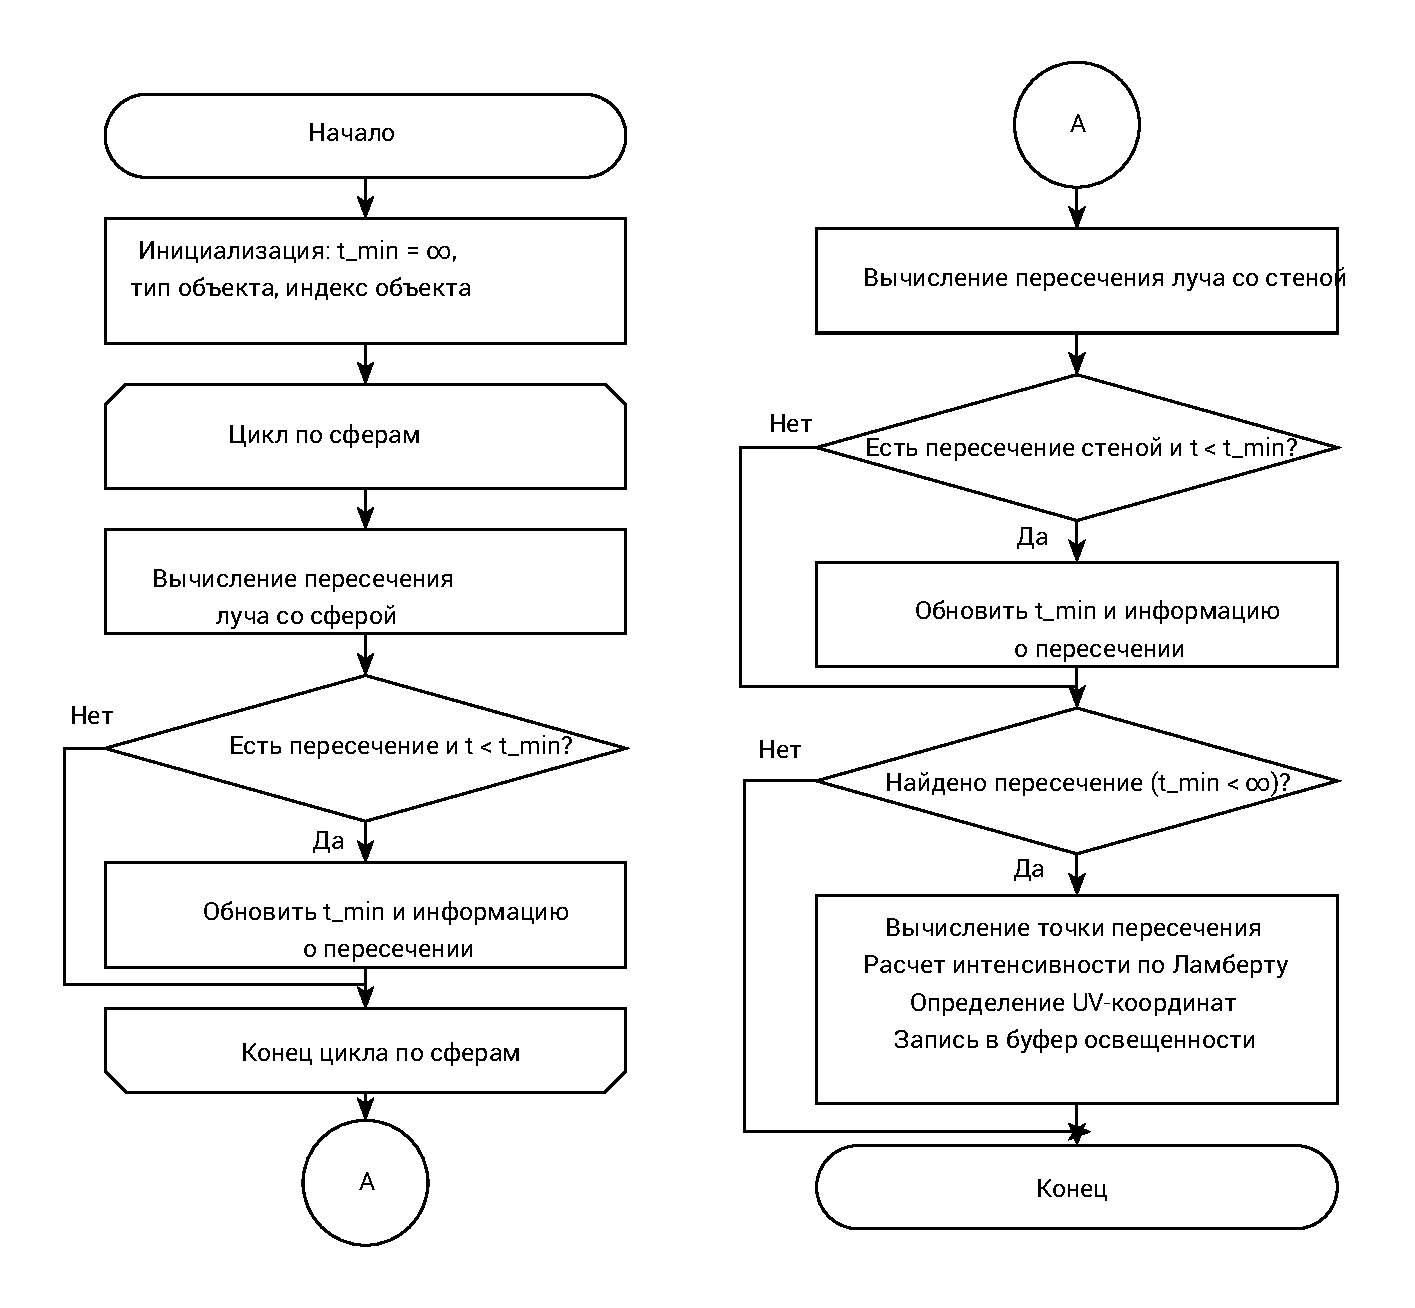
\includegraphics[width=0.9\textwidth]{images/algo_trace.pdf}
\caption{Схема алгоритма трассировки луча}
\label{fig:algo_trace}
\end{figure}

\subsubsection{Алгоритм обработки преломления в колпачке}

Моделирует прохождение луча через защитный колпачок (две концентрические сферы).

Входные данные: Входящий луч, конфигурация колпачка.

Выходные данные: Обработанный луч (или отсутствие, если интенсивность слишком мала).

\begin{figure}[H]
\centering
% Здесь будет вставлена блок-схема алгоритма обработки преломления в колпачке
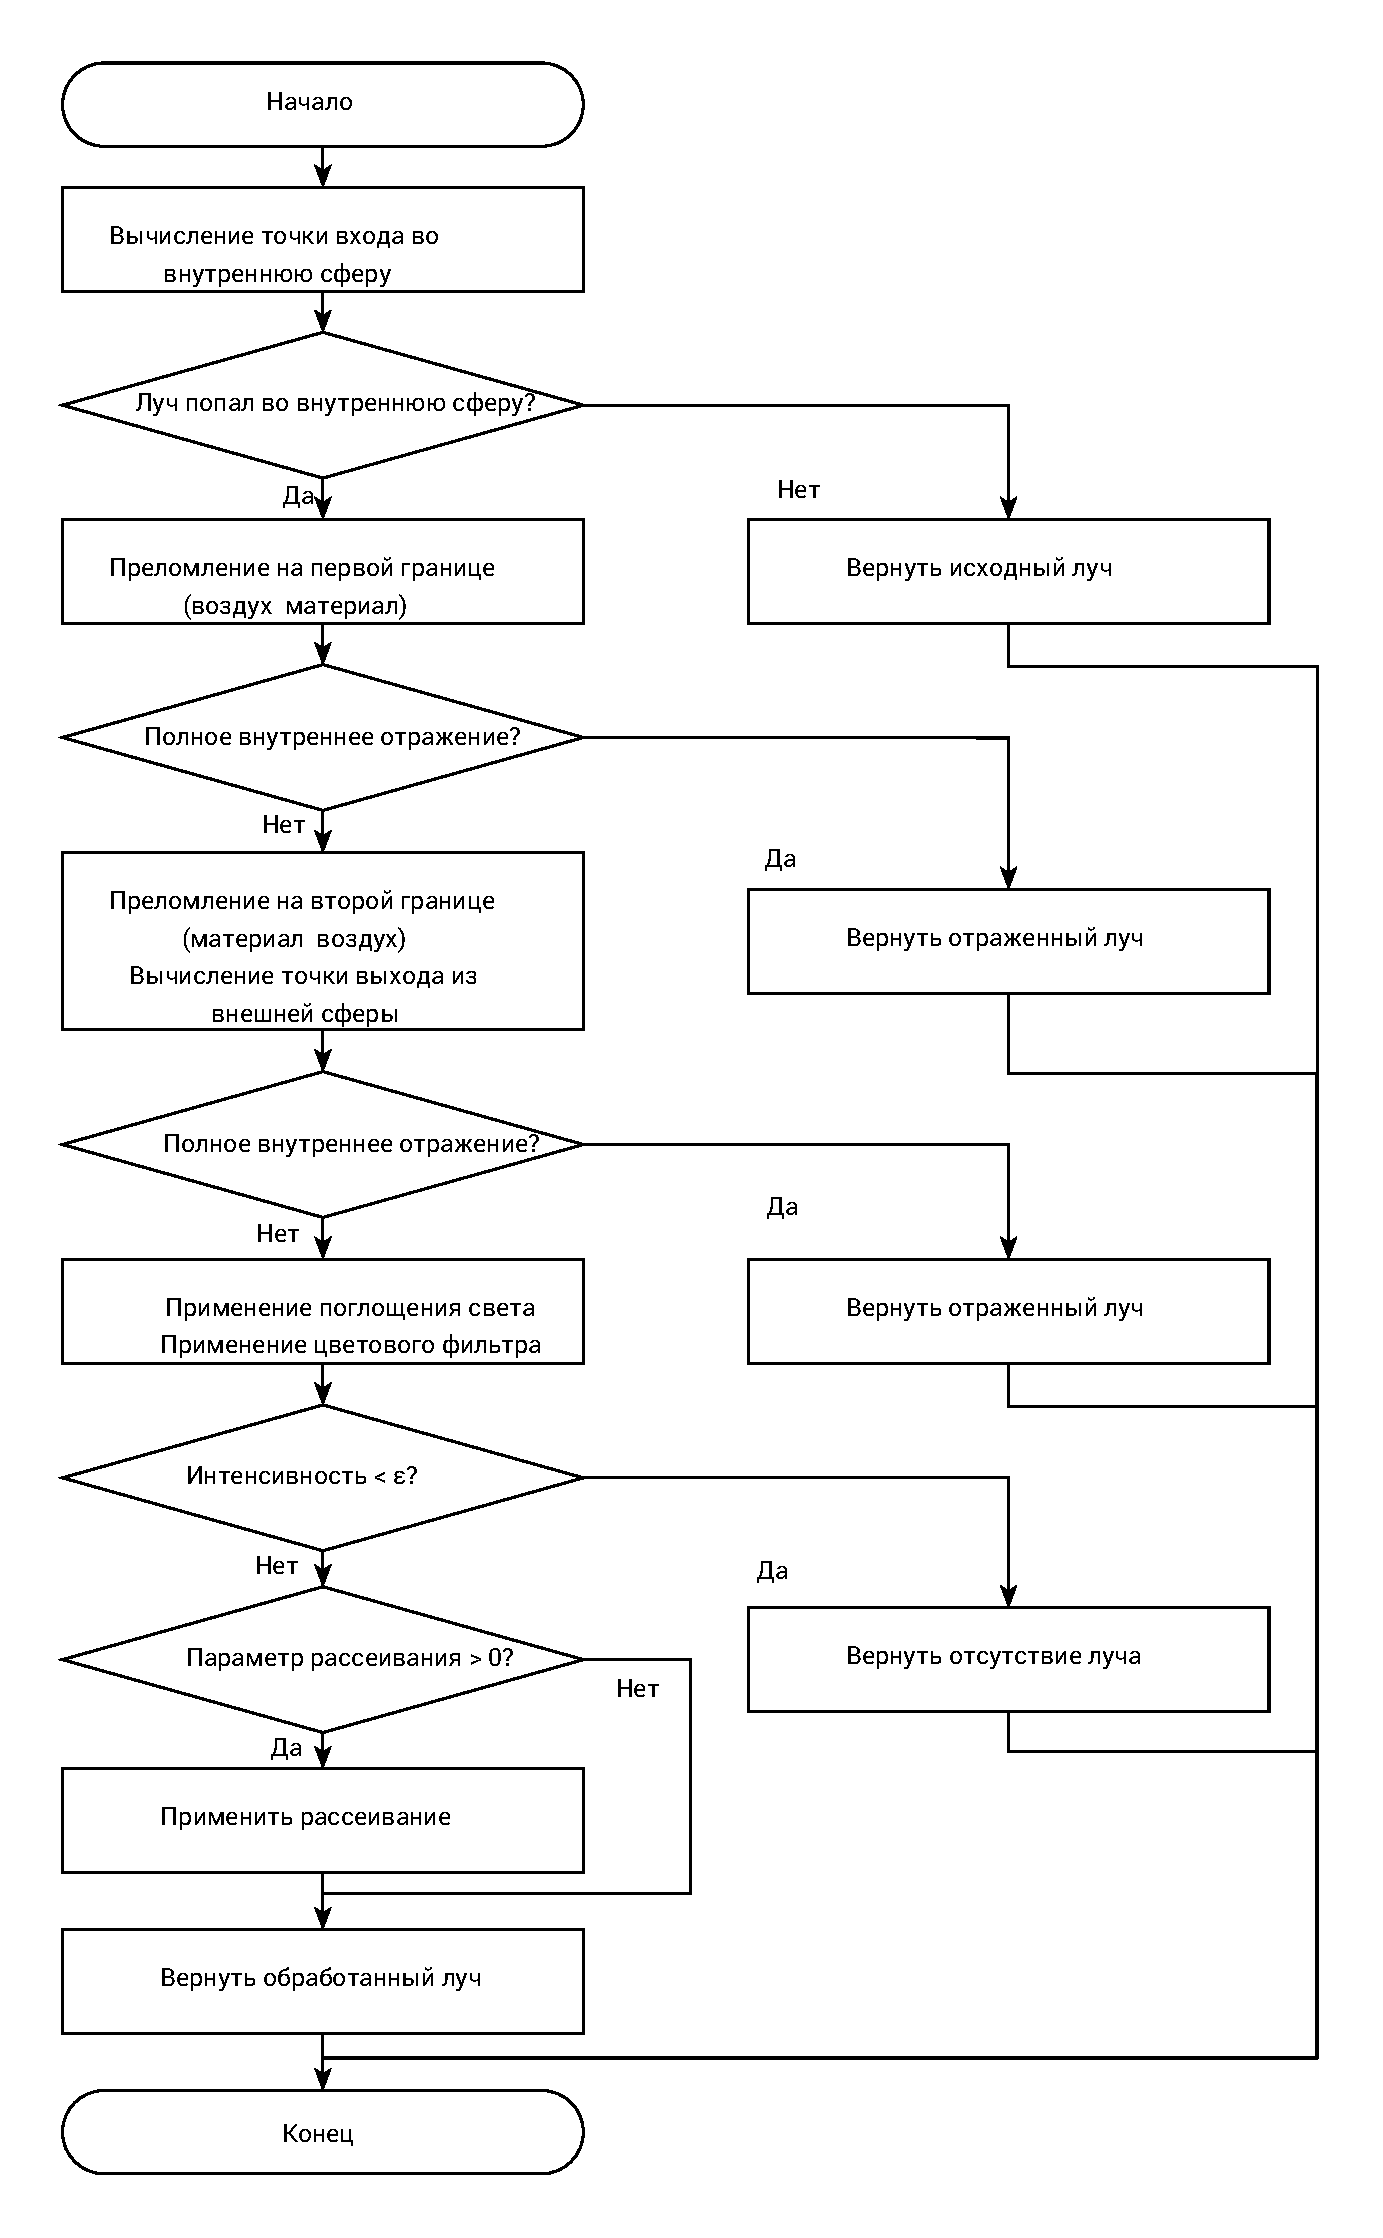
\includegraphics[width=0.9\textwidth]{images/algo_refract.pdf}
\caption{Схема алгоритма обработки преломления в колпачке}
\label{fig:algo_refract}
\end{figure}

\subsubsection{Алгоритм визуализации вида камеры}

Выполняет прямую трассировку лучей от камеры с использованием предрассчитанных карт освещенности.

Входные данные: Параметры камеры, предрассчитанные карты освещенности, конфигурация объектов сцены.

Выходные данные: Изображение сцены.

\begin{figure}[H]
\centering
% Здесь будет вставлена блок-схема алгоритма визуализации вида камеры
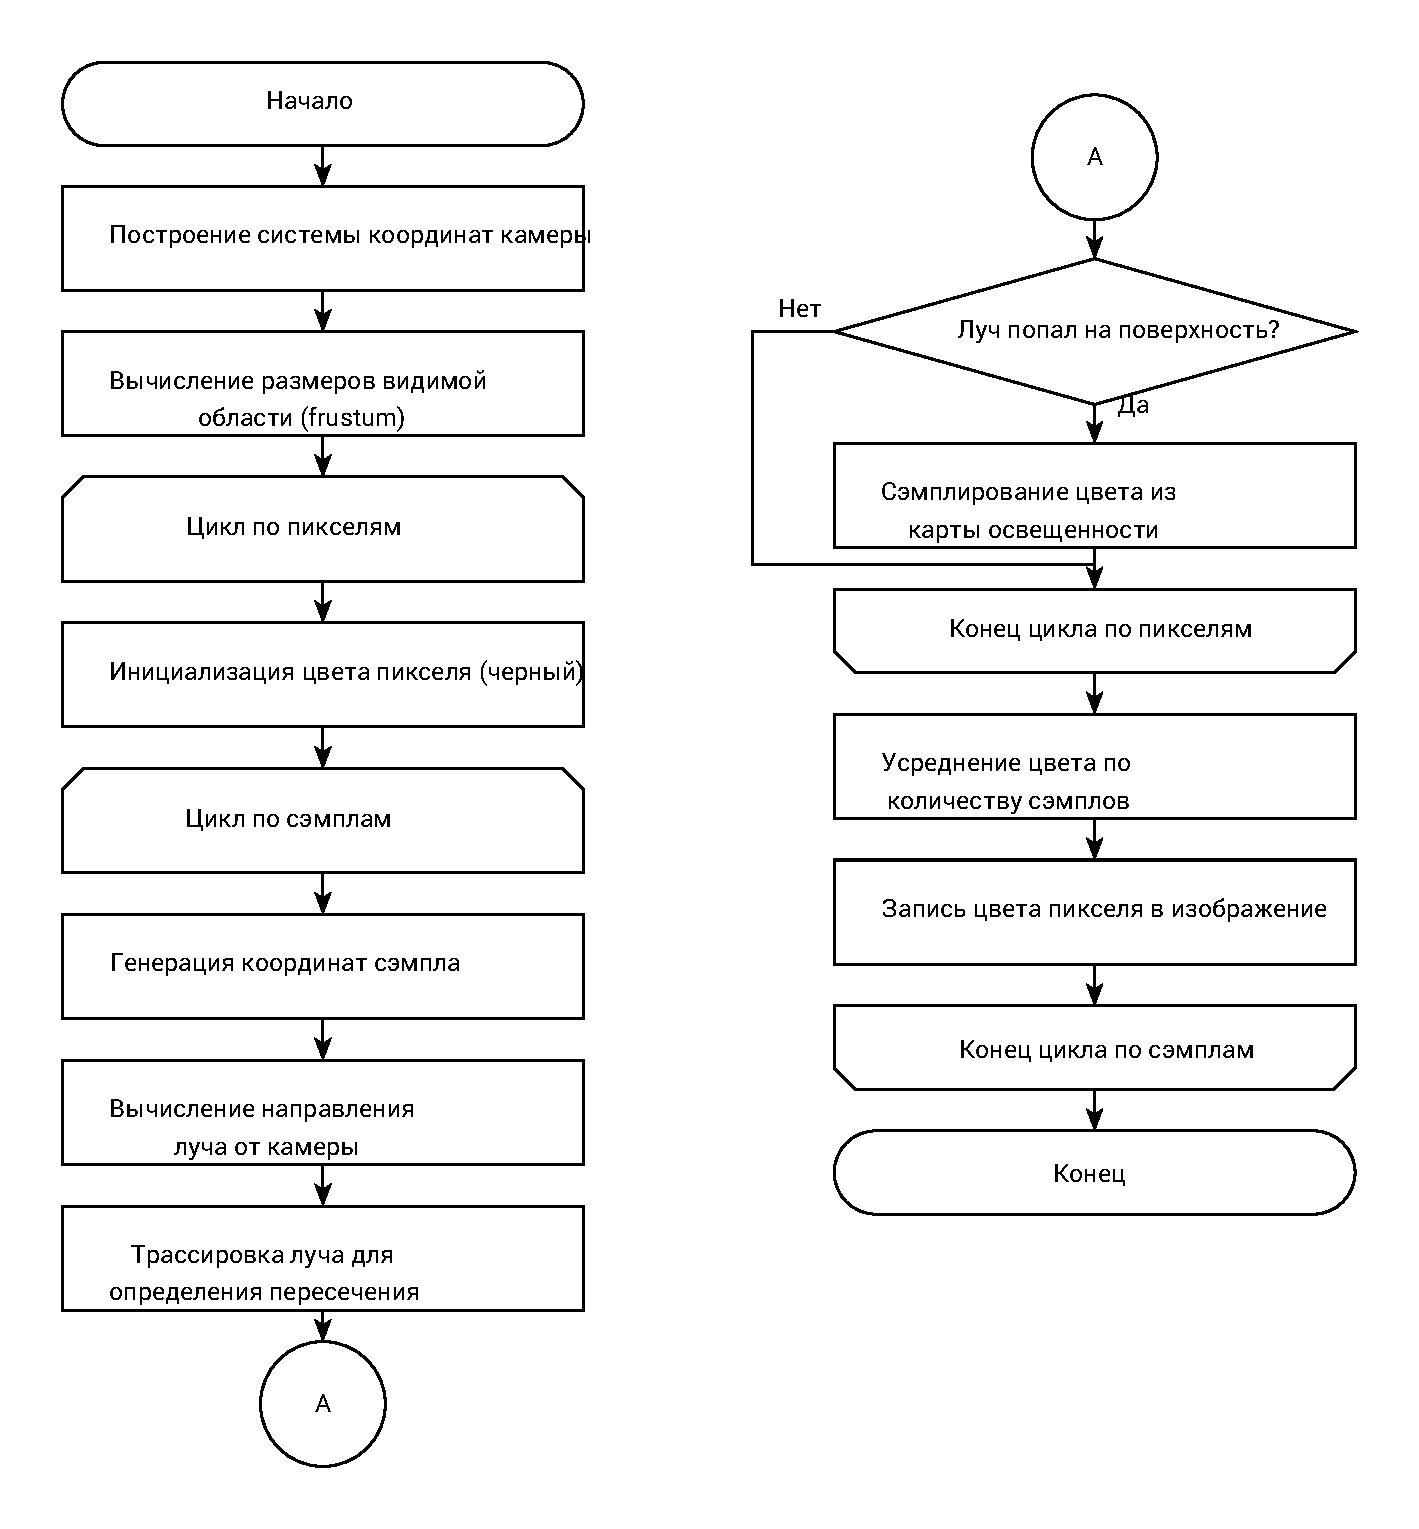
\includegraphics[width=0.9\textwidth]{images/algo_render.pdf}
\caption{Схема алгоритма визуализации вида камеры}
\label{fig:algo_render}
\end{figure}

\subsubsection{Алгоритм распределения направлений лучей}

Генерирует набор единичных векторов для равномерного покрытия телесного угла источника света.

Входные данные: Количество лучей $N$, метод распределения (стратифицированная сетка или решетка Фибоначчи).

Выходные данные: Массив из $N$ единичных векторов направлений.

\begin{figure}[H]
\centering
% Здесь будет вставлена блок-схема алгоритма распределения направлений лучей
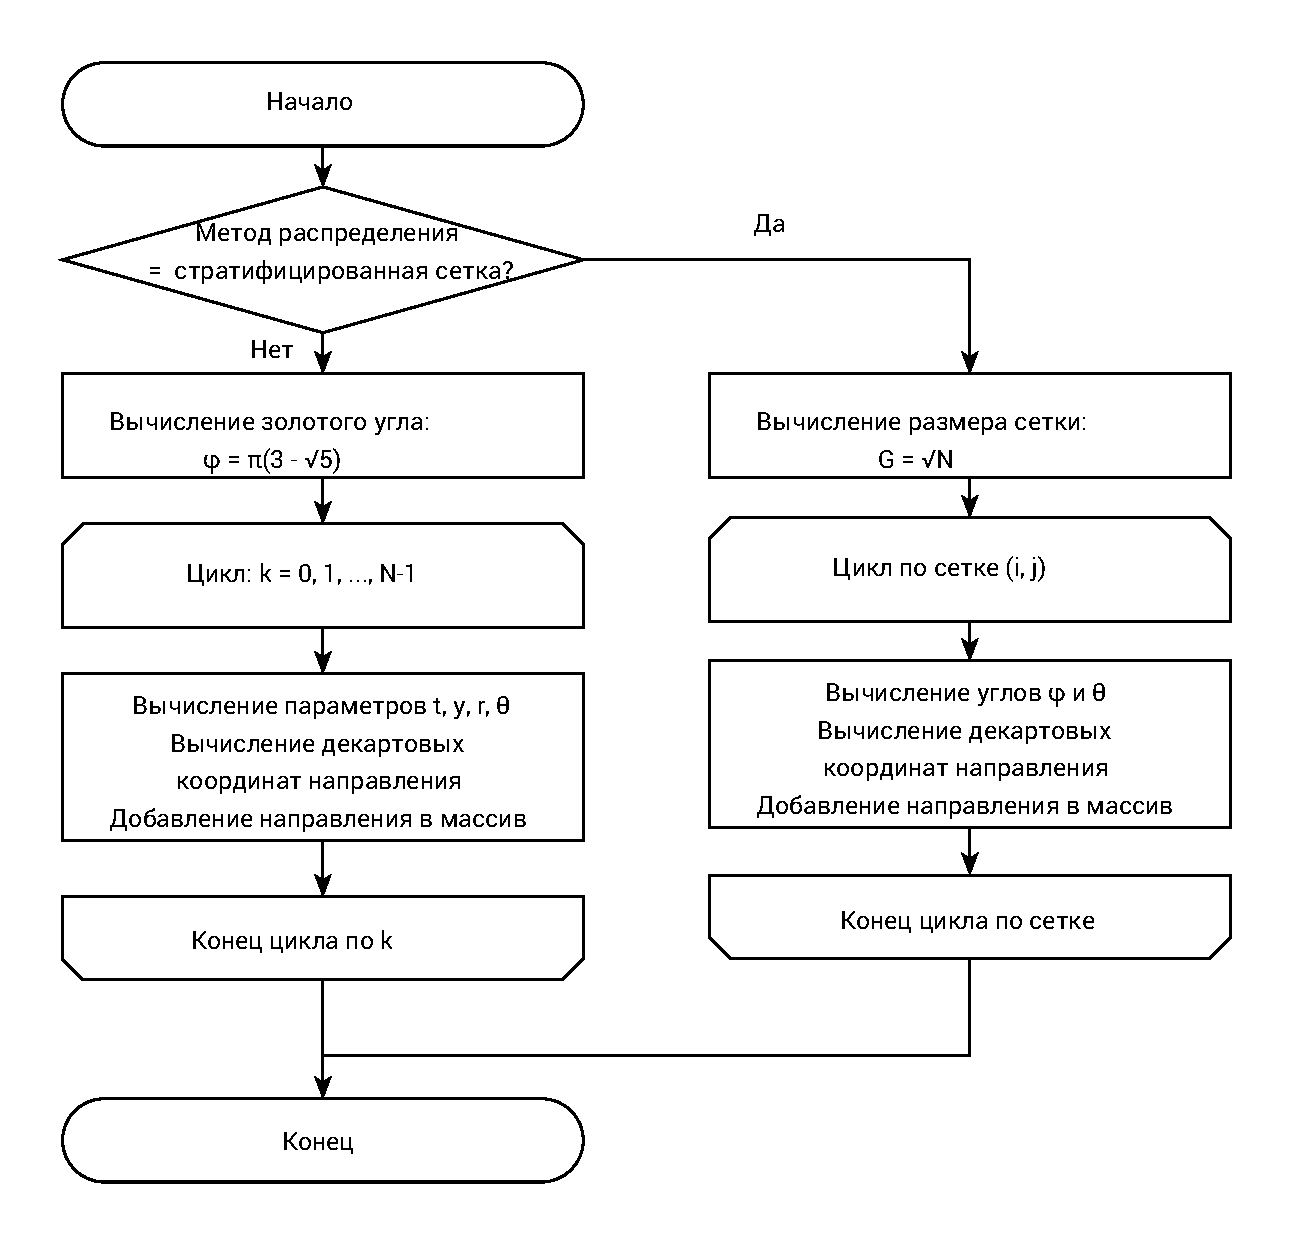
\includegraphics[width=0.9\textwidth]{images/algo_distribution.pdf}
\caption{Схема алгоритма распределения направлений лучей}
\label{fig:algo_distribution}
\end{figure}

\section{Проектирование интерфейса (UI/UX)}

\subsection{Описание взаимодействия пользователя с программой}

Пользователь взаимодействует с программой через графический интерфейс, который предоставляет следующие возможности:

\begin{itemize}
    \item создание паттернов источников света (точка, линия, дуга, круг) через панель инструментов;
    \item редактирование параметров источников света (позиция, цвет, интенсивность) через панель свойств;
    \item настройка параметров защитных колпачков (коэффициент преломления, прозрачность, рассеивание) через панель свойств;
    \item добавление объектов сцены (сферы) через меню или панель инструментов;
    \item запуск предварительного расчета освещения через кнопку "Рассчитать освещение" или "Bake Lighting";
    \item интерактивное управление камерой для просмотра результатов с разных ракурсов (перетаскивание мышью для вращения, колесико для масштабирования);
    \item просмотр результатов расчета в области визуализации;
    \item сохранение и загрузка конфигураций сцен через меню "Файл".
\end{itemize}

Основные сценарии использования: создание паттернов источников света, редактирование параметров источников и колпачков, добавление объектов сцены, запуск расчета освещения, просмотр результатов с управлением камерой, сохранение и загрузка сцен.

\subsection{Структура интерфейса}

Главное окно приложения содержит следующие элементы:

\begin{itemize}
    \item меню и панель инструментов --- обеспечивают доступ к основным функциям программы;
    \item панель создания паттернов --- содержит инструменты для создания паттернов источников света (точка, линия, дуга, круг) и поля ввода параметров паттерна (количество источников, размеры, расположение);
    \item панель редактирования параметров --- позволяет редактировать параметры выбранных источников света, защитных колпачков и объектов сцены;
    \item область визуализации --- отображает результаты расчета освещения и позволяет интерактивно просматривать сцену;
    \item панель управления камерой --- содержит элементы управления для изменения положения и ориентации камеры.
\end{itemize}


\clearpage
